\chapter{Firmware Architecture}

\section{Overview}
The firmware for the system is implemented on Texas Instrument's TMS320C5515 DSP in C and assembly using Code Composer Studio IDE. TI provides DSP/BIOS (in later versions called SYS/BIOS)  a real time operating system for their DSPs. These operating systems provides a wide range of system services to an embedded application such as preemptive multitasking, memory management and real-time analysis. The RTOS is feature rich and helps in quicker development and testing of firmware. But the very important of drawback of using the RTOS is the trade off of performance and controllability of the DSP for quicker development. For a resource and power constrained application, it is required to squeeze out the performance from the system which requires the firmware to have complete control over the underlying hardware. Thus firmware for the system is implemented on baremetal using  C and using the chip support library (CSL) for C5515 provided by TI. 


\vfill

The functions of Software could be categorized as the following:
 \begin{description}
 	\item[$\bullet$]
Initializing System and Sensors 
 	\item[$\bullet$]
Data collection
 	\item[$\bullet$] and storage 
Power management 
 \end{description}

 \begin{figure}[h]
	\centering
	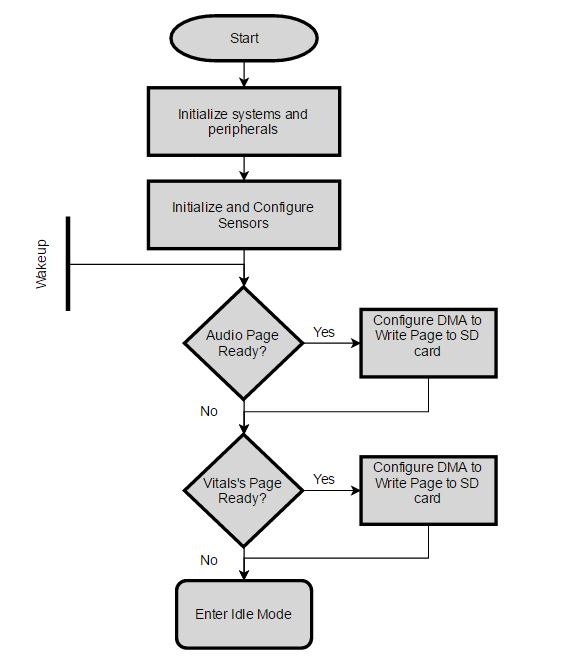
\includegraphics[scale = 1 ]{main.JPG}
	\caption{Main thread\label{main}}
\end{figure}

 \begin{figure}[h]
	\centering
	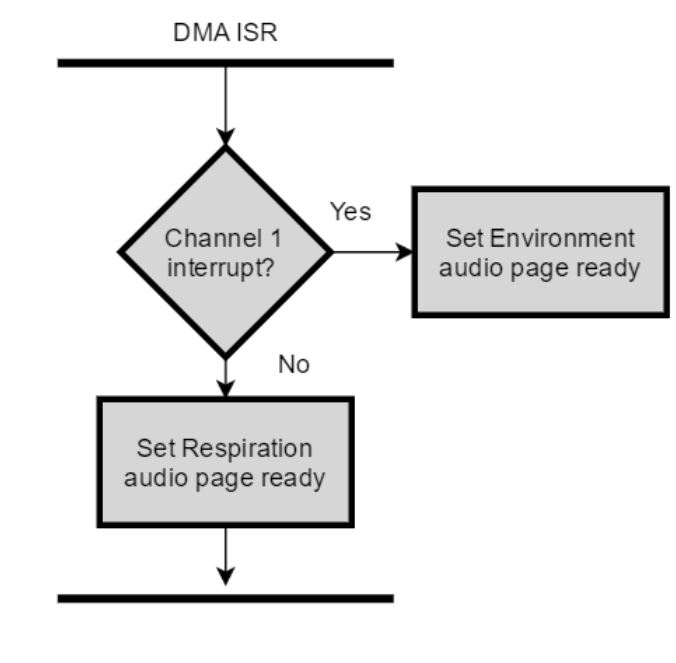
\includegraphics[scale = 0.5 ]{dma_interrupt.JPG}
	\caption{DMA Interrupt Service Routine\label{dma_isr}}
\end{figure}

 \begin{figure}[h]
	\centering
	\includegraphics[scale = 1 ]{ECG_interrupt.JPG}
	\caption{Hardware Interrupt Service Routine\label{ecg_isr}}
\end{figure}

\section{Initializing System}
First thing the firmware does after boot-up is to initialize the clock by configuring the PLL registers. PLL is configured to generate a 100 MHz clock to tick the system. After the clocks have been set up, the multiplexed I/O pins are configured to function as a specific peripheral or a input/output pins. Then the clock and power to those I/O pins and peripherals are enabled. After the I/O pins are configured, the communication peripherals such as SPI,I2C and I2S are configured. Their mode of operation(master or slave) , frequency of operation etc are initialized and configured. DSP's I2S module is configured as the I2S master(who supply bit clock and word clock) and the Audio codec AIC3204 is configured as the I2S slave. 

\section{Initializing sensor}
Audio Codec AIC3204 is configured, through the I2C interface , to sample the audio signal at 12Khz on each of the two channels and configured to amplify the signal with automatic gain correction feature enabled. The codec is also configured to filter the audio signal using first order IIR filter and 5 BiQuad filters to improve the audio quality. 

The ECG analog front end ADS1292R is configured to sample ECG signal at 500 samples per second. ADS1292R is configured to generate a hardware interrupt to inform the DSP when the sample is ready so that DSP can read the data using SPI interface. The ECG data is again stored in a ping-pong buffer and the data is stored in the permanent storage with the same mechanism as mentioned earlier. 
The environment temperature sensor STS21 is configured to sample the temperature with a 11bit precision. This data is acquired by polling. For every 500 ECG interrupt the STS21 is polled once to collect the temperature data.  
The Analog to Digital converters on board are configured to  sample the body temperature once for every 500 interrupt of ECG.

\section{Data Collection and storage}
The firmware is designed for concurrent data acquisition using dedicated hardware resources for the signals of interest. These hardware resources can perform certain required but  very defined functionalities like data buffering, filtering and data moving  without the intervention of the DSP. These hardware accelerators requires the DSP to configure for them to operate. The designed firmware is primarily preemption based where the DSP configures, assigns work, to the peripherals and hardware accelerators to concurrently acquire the signals.Upon completion of the assigned work , I.e data acquisition, these accelerators interrupt the DSP and the DSP configures DMA to write the collected data into the SD card. These sequence of interrupts and services happens periodically to acquire and store the signals.


\hspace{10mm} There are two non-mask able interrupts that preempts the DSP. One is the DMA interrupt, generated upon acquisition of audio signal of preconfigured size  and other one is the hardware interrupt generated by the ECG frontend signaling that the ECG data is ready. The following flow chard gives the functionality of DMA ISR and the hardware interrupt ISR.The ECG ISR is responsible of acquiring the available ECG data from the front end and also for acquiring the body and the environment temperature and accelerometer data.
 
 The following would provide insight and explain in detail the above mentioned mechanism with the context of audio signal acquisition .There are primarily two audio channels that are sampled at a very high frequency of 12 KHz. The audio signal acquisition and storage is the most intensive task of the entire system and also very power hungry task. Involving DSP to do the complete task would completely utilize the DSP's computational bandwidth allowing no space for DSP to do other useful work and also the overhead of doing this operation through DSP is very high.  TMS320C5515 includes 4 DMA controllers with four DMA channels each. It can move data among internal memory, external memory, and peripherals without intervention from the DSP and in the background of DSP operation. So DMA data transfer is used in audio signal collection and storing.  The following diagram shows the DMA in the DSP 
 \begin{figure}[h]
 	\centering
 	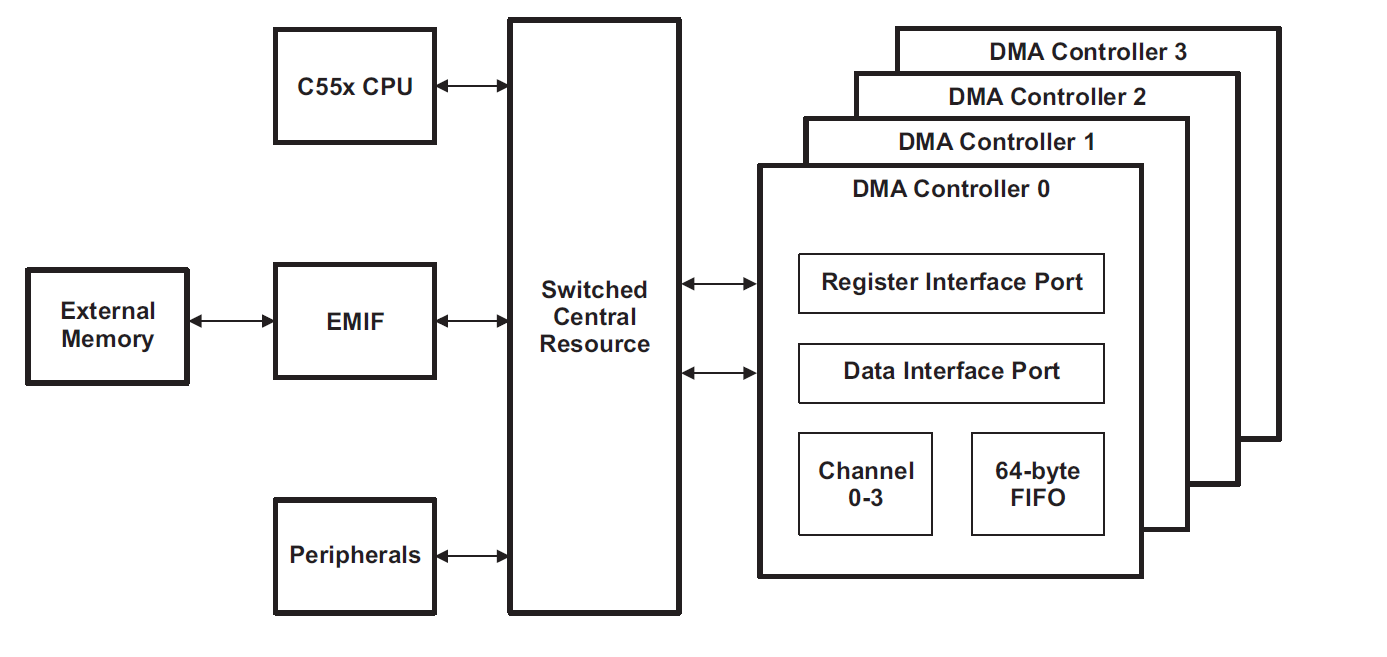
\includegraphics[scale = 0.5 ]{DMA_overview.PNG}
 	\caption{Conceptual Block Diagram of DMA controller\label{DMA_Architecture}}
 \end{figure} 
 The DMA is configured to collect the audio signal from the I2S peripheral and move it to SD card.The I2S receive event triggers the DMA to collect the audio signal. When the DMA fills up the allocated buffer it interrupts the CPU and the DSP initiates the SD card write using  other DMA channels and DMA takes care of the further action. The system continues acquiring audio signals even while writing data into the SD card . This is done through using DMA in ping-pong mode. The following diagram shows the ping pong operation mode.
  \begin{figure}[h]
 	\centering
 	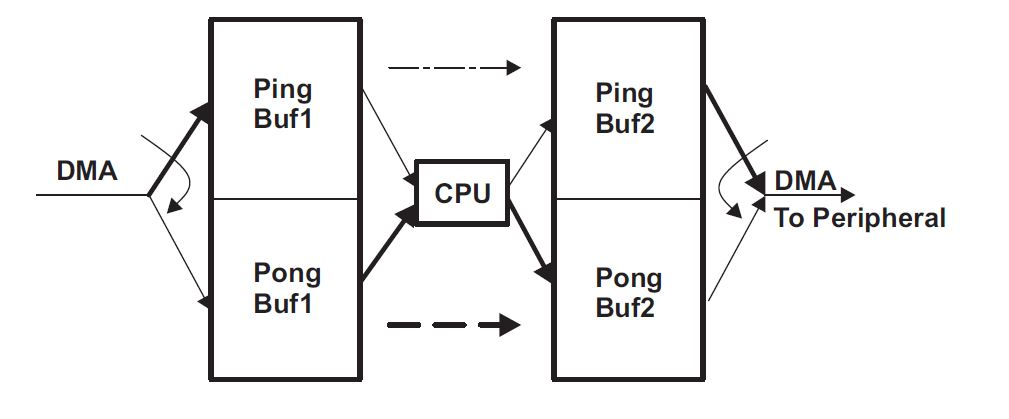
\includegraphics[scale = 0.5 ]{ping_pong.JPG}
 	\caption{Ping-Pong Mode for DMA Data Transfer\label{ping_pong}}
 \end{figure}
 When the ping buffer data is being copied to the SD card , the DMA acquires the incoming data and fills it in the pong buffer. So DMA used in ping-pong mode enables the system to collect the audio signals and store the previously cached signal simultaneously. 
 
 As mentioned earlier the measurement of temperature signal is triggered for every 500 interrupts of ECG. This adds a overhead of checking if the interrupt count every time ECG interrupt is serviced. The measurement of temperature from the context of ECG interrupt increases the worst case execution time of the ISR which is not preferred in general for typical application. One could argue that the system could have used a timer and generate a timer interrupt every one second and trigger the temperature measurement instead of tightly coupling it with the ECG ISR. The reason for not going with this approach is the cost in terms of power for running a dedicated timer for the temperature measurement. Power is the most scarce resource in the system and that is the important reason why the former method is chosen than the latter one. As long as the tasks could be finished on available clock cycles without disturbing other functionality of the system, it is fine even if the worst case execution time of the ISR increases.
 \begin{figure}[h]
 	\centering
 	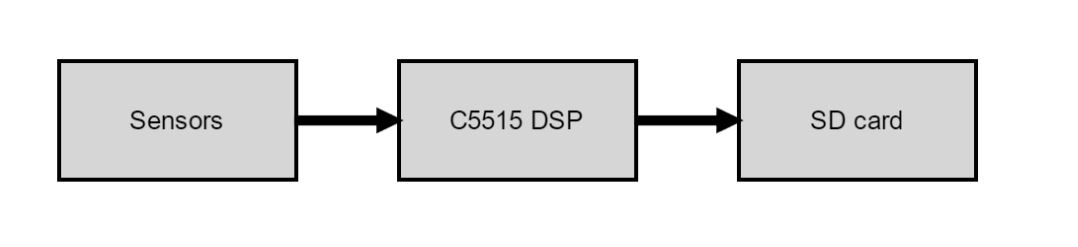
\includegraphics[scale = 0.5 ]{record_dataflow.JPG}
 	\caption{Flow of data in during record\label{record_datalow}}
 \end{figure}

\subsection{Importing the Data}
Once the data has been saved to the micro SD card and testing is complete, it can be read directly by a computer. A custom file system is used to store the data, so it can not be directly recognized on a computer. A filesystem driver for the custom filesystem is developed in python, which could parse the data in the SD card and create files of each of the signals. These files are read by a MATLAB script that does post processing and generates data vectors corresponding to each signal. For example in case of body temperature sensor, the data in the file is the raw ADC values, the calibration details of the body temperature is embedded into MATLAB code , so it does convert raw ADC temperature  data into a meaningful value through the calibration information.  
MATLAB plots the data and visualizes it in such a way that the user can relate and see all the signals together and it allows user to jump into the time of interest. 
 \begin{figure}[h]
	\centering
	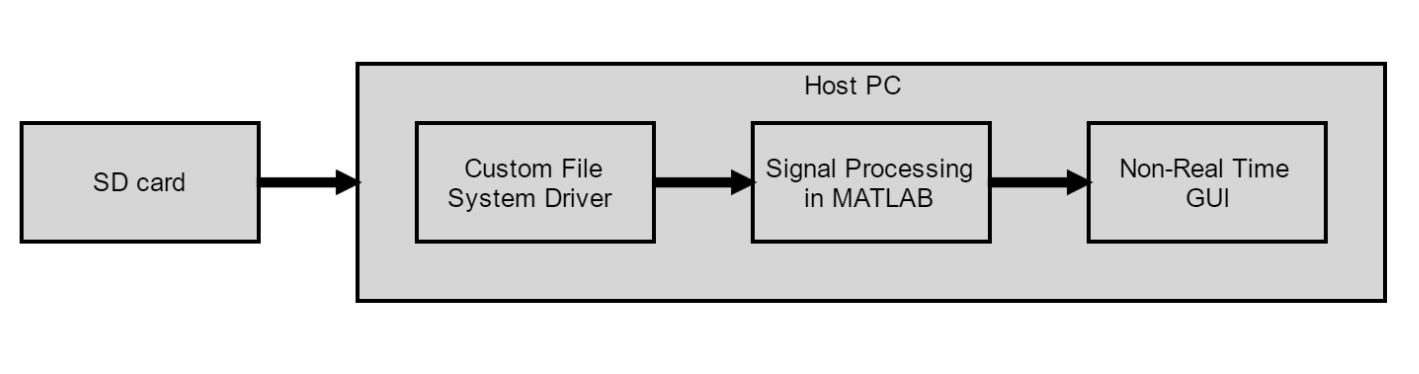
\includegraphics[scale = 0.5 ]{play_dataflow.JPG}
	\caption{Flow of data in import record\label{play_dataflow}}
\end{figure}